\documentclass[12pt,letterpaper]{article}
\usepackage[utf8]{inputenc}
\usepackage[T1]{fontenc}
\usepackage{lmodern}
\usepackage[margin=1in]{geometry}
\usepackage{amsmath,amssymb,amsthm}
\usepackage{graphicx,booktabs,multirow,array}
\usepackage{caption}
\usepackage{listings}
\usepackage{setspace}
\usepackage[hidelinks,hypertexnames=false]{hyperref}

\onehalfspacing
\graphicspath{{figures/}}
\captionsetup{font=small,labelfont=bf}
\lstset{basicstyle=\ttfamily\scriptsize,breaklines=true,columns=fullflexible,
  keepspaces=true,upquote=true,showstringspaces=false}

% Table and figure numbers follow the French original, including Tables 6.1
% and 6.2 and Figure 6.1, which sit in section 5 there.
\newcommand{\numtable}[2]{\renewcommand{\thetable}{#1}\caption{#2}\addtocounter{table}{-1}}
\newcommand{\numfigure}[2]{\renewcommand{\thefigure}{#1}\caption{#2}\addtocounter{figure}{-1}}
\newcommand{\Et}{E_t}
\newcommand{\gbar}{\bar{g}}
\newcommand{\abar}{\bar{\alpha}}
\newcommand{\dtilde}{\tilde{\delta}}
\newcommand{\Theg}{\Theta_g}
\newcommand{\Thec}{\Theta_c}
\newcommand{\Thek}{\Theta_k}
\newcommand{\Thet}{\Theta_\tau}
\newcommand{\Phir}{\Phi_r}
\newcommand{\T}{\mathbb{T}}
\newcommand{\WW}{\mathcal{W}}
\newcommand{\TT}{\mathcal{T}}
\newcommand{\XX}{\mathcal{X}}
\newcommand{\DD}{\mathfrak{D}}
\newcommand{\pif}{\pi}

\begin{document}

\begin{titlepage}
\centering
{\large HEC MONTR\'EAL\par}
\vspace{2cm}
{\LARGE\bfseries Government Spending, Financing Method, and the Fiscal Multiplier in a Liquidity Trap\par}
\vspace{1cm}
by\par
\vspace{0.3cm}
{\large Aaron Isra\"el\par}
\vspace{1.5cm}
Management Sciences\par
(Applied Economics Option)\par
\vspace{1.5cm}
Thesis submitted in view of obtaining the degree of\par
Master of Science in Management (M.Sc.)\par
\vspace{1.5cm}
November 2023\par
\copyright{} Aaron Isra\"el, 2023\par
\vfill
{\small \textbf{Unofficial English translation.} The official version is the French thesis,
\emph{D\'epenses publiques, mode de financement et multiplicateur budg\'etaire en trappe \`a liquidit\'e},
HEC Montr\'eal, 2023, available as \texttt{paper/thesis\_fr.pdf} in this repository.\par}
\end{titlepage}

\pagenumbering{roman}
\setcounter{page}{3}

\section*{Abstract}
\addcontentsline{toc}{section}{Abstract}

The aim of this thesis is to study how the financing method of a fiscal stimulus plan affects the government spending multiplier in different cyclical contexts, namely in normal times and in a liquidity trap, the latter scenario referring to a situation in which the nominal interest rate is stuck at its lower bound of zero. To do so, we develop a dynamic general equilibrium model of a closed economy in which government spending is split between operating expenditure (consumption) and investment and is financed by a lump-sum tax, by a tax on labor income, or by debt.

We begin by deriving analytical results in a stylized version of the model, obtained through certain simplifying assumptions. In particular, we assume that the duration of the liquidity trap is exogenous and that the stimulus plan (and the resulting tax increase) ends as soon as the economy has exited the trap. This model indicates that the fiscal multiplier of a stimulus plan financed by a tax on labor income is larger than that associated with lump-sum tax financing in a liquidity trap. By simulating the more general version of the model, however, we show that when the government balances its budget at all times, lump-sum tax financing invariably generates the highest multiplier, especially when the stimulus plan consists of consumption spending. This is because the inflationary effect of the income tax persists even once the economy has exited the trap. By contrast, when the stimulus plan is initially financed by public debt, the fiscal multiplier is larger the more aggressively the labor income tax adjusts to repay the debt, thereby approaching the multiplier associated with lump-sum tax financing.

\medskip
\noindent\textbf{Keywords:} Fiscal multiplier, liquidity trap, Ricardian equivalence, monetary policy, government consumption, public investment

\newpage
\tableofcontents
\newpage
\listoftables
\listoffigures

\section*{Translator's note}
\addcontentsline{toc}{section}{Translator's note}

This translation keeps the content, numbering, tables, and printed values of the French thesis. Apparent errors in the original are left as printed and are listed in \texttt{docs/errata.md}. Figures were redrawn in English from a rerun of the model, in the same panel layout as the original. Annex B reproduces the original code listings with their comments translated.

\section*{Acknowledgements}
\addcontentsline{toc}{section}{Acknowledgements}

I wish to thank my thesis supervisor, Hafedh Bouakez, most warmly for his unfailing support throughout this academic adventure. His enlightened advice and sharp expertise were of capital importance in the design and completion of this thesis.

I also wish to express my deep gratitude to my family. Your encouragement gave me the strength to persevere in the face of challenges and reminded me of the importance of pursuing my goals with determination.

\newpage
\pagenumbering{arabic}

\section{Introduction}

The effectiveness of government spending in stimulating economic activity has always been an important subject of debate among researchers and policymakers. This debate in fact goes back to the 1930s, when the British economist John Maynard Keynes developed his general theory of employment, interest and money.

Keynes suggested that in periods of economic recession, the state should intervene to stimulate economic activity by increasing government spending. According to Keynes, this policy would have a multiplier effect on the economy because it would stimulate aggregate demand, which would in turn create jobs and stimulate economic growth (Keynes 1936). Fiscal policy can thus prove to be a formidable tool when monetary policy becomes ineffective in a so-called classical recession, that is, negative growth with little inflation or even deflation. Several major stimulus plans have marked history, such as the New Deal of 1930 in response to the Great Depression, the Marshall Plan for Europe after the Second World War, or more recently the stimulus plans to fight the negative effects of the COVID-19 pandemic.

A vast scientific literature has thus developed in an attempt to grasp the factors that influence multipliers, from both a theoretical and an empirical point of view. In this thesis, the main factors of interest are the cyclical context, particularly that of the liquidity trap (i.e.\ when the nominal interest rate is stuck at its lower bound of 0), and the method of financing government spending during a fiscal stimulus plan.

Our study is based on a New Keynesian dynamic stochastic general equilibrium (DSGE) model that incorporates monopolistic competition and nominal price rigidity. This class of models is considered an extension of real business cycle (RBC) models, in which monetary policy plays no important role since money is neutral at all times. Our model is that of a closed economy in which government spending is split between operating expenditure (consumption) and investment and is financed by a lump-sum tax, by a tax on labor income, or by debt. The model draws on the work of Bouakez, Guillard and Roulleau-Pasdeloup (2017, 2020), but extends it by introducing a distortionary tax on labor income and public debt.

The contribution of this thesis is to assess the differences in the size of the multiplier that are due exclusively to differences in the financing method of the fiscal stimulus plan, for both government consumption and public investment. To do so, we consider various scenarios that share a common steady state, so that only spending away from the steady state is financed differently. This counterfactual exercise has rarely been carried out in the literature. Moreover, the fact that it is performed in a model with microeconomic foundations and rational expectations makes it immune to the Lucas critique (Lucas, 1976).

We begin by considering a stylized version of our model, obtained by imposing restrictive assumptions that allow us to solve the model algebraically (up to a first-order approximation). In particular, we assume that the duration of the liquidity trap is exogenous and that the stimulus plan (and the resulting tax increase) ends as soon as the economy has exited the trap. We thus obtain an algebraic expression for the multiplier both under lump-sum tax financing and under labor income tax financing. Our results indicate that although the multiplier is higher in normal times in the first case, this result reverses when the economy is in a liquidity trap, with labor income tax financing making the stimulus plan even more expansionary. This holds whatever the composition of the stimulus plan (in terms of consumption and investment spending).

The intuition behind these predictions lies in the fact that the labor income tax is inflationary, since it reduces labor supply (hence its distortionary nature). In normal times, this amplifies the increase in the nominal and real interest rates, thereby reducing the effect on consumption and hence the fiscal multiplier relative to the case in which financing takes place through a lump-sum levy. In a liquidity trap, since the nominal interest rate is stuck at its lower bound of 0, the inflationary effect of the distortionary tax further reduces the response of the real interest rate, thereby amplifying the multiplier. This mechanism holds regardless of whether the stimulus plan consists of consumption or investment spending.

We then relax the restrictive assumptions of the simplified version and consider a more general version that we solve non-linearly. In this version, the exit from the trap is endogenous and the inflationary effect of the labor income tax persists even once the economy has exited the trap. In an economy where the government balances its budget at all times, this implies that lump-sum tax financing invariably generates the highest multiplier in normal times and in a trap. This is all the more true when the stimulus plan consists of consumption spending. By contrast, when the stimulus plan is initially financed by public debt, the more aggressively the labor income tax adjusts to repay the debt, the larger the multiplier, thereby approaching the multiplier associated with lump-sum tax financing, especially when the stimulus plan consists of investment spending and the time to build public capital is long.

The rest of this thesis is organized as follows. In Section 2, we review the literature on existing theoretical and empirical approaches to assessing the fiscal multiplier. Section 3 presents our theoretical model and the derivation of its equilibrium conditions. In Section 4, we present analytical results based on a simplified version of the model. In Section 5, we present results based on the general version of the model with and without debt. Section 6 concludes.

\section{Literature review}

\subsection{Theoretical approaches}

There is a vast theoretical literature on government spending multipliers in a liquidity trap. Most studies, however, have focused on fiscal stimulus plans centered on consumption spending and financed by a lump-sum tax.

Among the best-known works, we can first cite the article by (Christiano, Eichenbaum and Rebelo, 2011), in which the authors argue that the fiscal multiplier can be well above 1 when the nominal interest rate is set at its zero lower bound. In this situation, the inflationary pressures that result from a fiscal stimulus plan lead to a fall in the interest rate, so that the increase in government spending has a much greater impact on output and employment than it would in normal times. To support their argument, the authors develop a DSGE model inspired by Altig et al.\ (2011), in which they include a shock to the household discount factor and to government spending.

This conclusion is corroborated by Eggertsson (2011), who studies the effects of tax cuts and government spending increases in economic circumstances resembling those that characterized the 2008 crisis. He finds that in the presence of a very accommodative monetary policy (keeping the nominal interest rate at a very low level), a cut in taxes on labor and capital contracts economic activity, whereas a temporary increase in government spending has a large expansionary effect, much larger than in normal circumstances.

Finally, we can also cite the article by Woodford (2011), which describes the key factors that determine the size of the fiscal multiplier in a New Keynesian model. He shows that price or wage rigidity yields larger multipliers than in a neoclassical model, although the size of the multiplier depends crucially on the response of monetary policy. A multiplier well above 1 is possible when monetary policy is constrained by the zero lower bound, and in this case, welfare improves if government spending increases to partially fill the output gap that results from the inability of the monetary authorities to lower interest rates.

\subsubsection{Method of financing government spending}

As mentioned above, a large part of the literature assumes that government spending is financed by a lump-sum tax at all times, even during a government stimulus plan. The government thus has a balanced budget in each period, which implies that, in a general equilibrium macroeconomic model, the government budget constraint is not included among the equilibrium conditions. When lump-sum taxes are the only levies available, the balanced-budget assumption is not restrictive insofar as Ricardian equivalence holds. According to this proposition, first developed by David Ricardo in the early 19th century and later elaborated by Barro (1974), financing government spending through current or future lump-sum taxes will have equivalent effects on the economy. In the second case, the initial increase in spending is then financed by an increase in public debt.

This approach may be more convenient from a practical point of view, but it is nonetheless unrealistic: lump-sum taxes are never used to finance stimulus plans. The contribution of this thesis is to consider an alternative form of financing based on the labor income tax, with or without the possibility of public borrowing. Unlike the lump-sum tax, the labor income tax is distortionary. Ricardian equivalence therefore does not hold in this case.

Very few theoretical studies have examined the effects of government spending in a liquidity trap in the absence of Ricardian equivalence. Nakata (2017) shows that, regardless of the type of tax available and the initial level of debt, the optimal fiscal policy in response to an adverse shock is characterized by an increase in spending followed by a reduction below its initial level and an eventual return to it. However, the magnitude of the changes in government spending and their welfare implications depend strongly on the available fiscal instrument and the initial level of debt.

Aloui and Eyquem (2019) study the link between the size of public debt and the effectiveness of government spending in stimulating the economy in normal times and in a liquidity trap. They develop a New Keynesian model in which the liquidity trap is generated by a shock to the quality of private capital. Government spending is financed by taxes on labor income and capital income and by debt. In normal times, when the economy is characterized by high initial public debt (as a percentage of GDP), this tends to reduce the fiscal multiplier. By contrast, in a liquidity trap, high levels of public debt produce larger multipliers.

Lemoine and Lind\'e (2023), for their part, consider a wide range of fiscal instruments in a non-Ricardian model and show that in a liquidity trap, conventional fiscal policies (such as public spending on infrastructure) can be more effective than unconventional fiscal policies (such as a gradual increase in the sales tax combined with a cut in the labor income tax). This is particularly true when government credibility is low and the liquidity trap is caused by non-fundamental shocks, or when policymakers find it difficult to coordinate the adjustment of the sales tax with a substantial change in the labor income tax.

\subsubsection{Government consumption and investment spending in a liquidity trap}

Government spending can be broken down into consumption (or operating) spending and investment spending. The latter serves to increase the stock of public capital after a delay, often called ``time to build.'' One of the first articles to introduce public capital into a real business cycle model, subject to a time-to-build constraint, is Kydland and Prescott (1982). The authors show that the commonly used assumption of a time to build of a single quarter is inadequate to explain cyclical fluctuations in macroeconomic aggregates in the United States. They suggest that a time to build of several quarters is needed to do so. This assumption has thus been adopted in a large number of articles, including that of Bouakez, Guillard and Roulleau-Pasdeloup (2017), which will serve as our point of reference, notably in the construction of the model and in the analytical solution.

In that work, the authors study the effectiveness of public investment spending as a stimulus tool in a New Keynesian economy where a fraction of government spending increases the stock of public capital, itself subject to a time-to-build constraint. They highlight the importance of breaking down government spending into its consumption and investment components. In particular, they show that failing to account for the composition of a stimulus plan by neglecting its investment component would lead to a significant underestimation of the multiplier, especially in a liquidity trap.

Boehm (2020) also explains how important the allocation of government spending is for the size of the multiplier. The model he develops predicts that in normal times, the multiplier associated with public investment spending is smaller than that associated with government consumption, when spending changes are short-lived. Two equivalent explanations are proposed for this result. The first emphasizes that investment spending shocks have practically no effect on household labor supply, that is, they do not encourage households to work more. The second explanation highlights the fact that, because of greater intertemporal substitutability, private investment falls more after public investment spending shocks than private consumption does after government consumption spending shocks.

In the same vein, Ramey (2020) studies the short- and long-term effects of public investment on the economy. The theoretical analysis considers both neoclassical and New Keynesian models. Long-term multipliers of public investment depend essentially on the elasticity of the production function with respect to public capital and on the economy's initial position relative to the socially optimal level of public capital. Starting from a low level of capital with a high elasticity yields high multipliers. The author also finds that although public investment has significant long-term effects, short-term multipliers are generally lower than those of government consumption in normal times, because of construction delays and the propensity of public investment to crowd out private investment. The author notes, however, that there is both theoretical and empirical support for the idea that the short-term multiplier of public investment is higher when interest rates are at the zero lower bound. The theoretical mechanisms that lead to this effect imply that financing government spending through income taxes, rather than through deficits, leads to higher multipliers.

Finally, Bouakez, Guillard and Roulleau-Pasdeloup (2020) examine optimal fiscal policy in an economy plunged into a deep recession characterized by a liquidity trap, in which the government can allocate its spending to public consumption and investment, the latter increasing the stock of public capital under a time-to-build constraint. The results of the study suggest that the optimal response to such a shock is to increase government spending and change its composition by raising the share of investment spending.

\subsection{Empirical approaches}

There is also a very large literature that sets out to estimate fiscal multipliers empirically. The abundance of existing work, however, makes it impossible to review it exhaustively in a limited space. Ramey (2019) examines the state of recent knowledge on the subject based on empirical estimates carried out in the decade following the 2008 crisis. The estimates surveyed lie mainly in a narrow range from 0.6 to 1. However, this range widens when specific national characteristics are taken into account, such as the exchange rate regime and the type of government spending. In the next subsections, we therefore present the articles that are most influential and closest to the concerns of this thesis.

\subsubsection{Estimating the multiplier by type of government spending}

Perotti (2004) was the first to use a structural VAR to compare the macroeconomic effects of the three main categories of government spending: investment, consumption, and transfers to households, both in terms of the size and the speed of their effects on GDP and its components. Spending shocks are identified through a Cholesky decomposition of the variance-covariance matrix of the statistical residuals. His results do not support the conclusion that public investment shocks are more effective than government consumption shocks in stimulating GDP. This is true both in the short term and, perhaps more surprisingly, in the long term. In fact, government investment seems to discourage private investment, particularly in housing and in machinery and equipment.

Bouakez, Larocque and Normandin (2018) undertake a disaggregated analysis of the effects of government spending on economic activity in the United States, breaking down public consumption and investment into various subcategories. For each subcategory, the authors estimate a structural vector autoregression in which government spending shocks are identified by exploiting the conditional heteroskedasticity of the structural disturbances, which makes it possible to relax the identifying restrictions commonly used in the literature. The spending categories that yield the largest multipliers (above 1) are purchases of durable goods and investment in structures. The results also suggest that there is little relationship between the importance of a category of government spending and the magnitude of its effect on aggregate output.

Boehm (2020) also compares the multipliers associated with public consumption and investment using OECD panel data from 2003 to 2016. His methodology is based on the local projections of Jord\`a (2005), and the multipliers are obtained by drawing on the approach of Ramey and Zubairy (2018). The empirical results broadly support the predictions of his theoretical model. First, the multiplier associated with public investment spending is smaller than that associated with government consumption spending. Second, the difference between these two multipliers is due to a large crowding-out effect on private investment, caused by a rise in the real interest rate specific to the investment goods sector.

\subsubsection{Estimating the multiplier conditional on the business cycle}

Some empirical work has estimated the multiplier by taking the cyclical state of the economy into account. These studies set out to determine whether the fiscal multiplier varies according to whether the economy is in recession or expansion. We can cite the study by Auerbach and Gorodnichenko (2012), who use a regime-switching econometric model to assess the multiplier in recession and in expansion using U.S.\ data. They find large differences in the size of spending multipliers in these two phases of the cycle, with fiscal policy being considerably more effective during recessions. More specifically, the authors obtain a multiplier between 0 and 0.5 in expansion, and between 1 and 1.5 in recession.

Similarly, Ramey and Zubairy (2018) try to determine whether the fiscal multiplier is higher during periods of economic slowdown or when nominal interest rates are close to the zero lower bound. Using new quarterly historical U.S.\ data covering several major wars and deep recessions, the authors estimate multipliers that are positive but below 1, regardless of the degree of slack in the economy. These results are robust to two main identification schemes, two different estimation methodologies, and many alternative specifications. By contrast, the results are more mixed for the zero lower bound on the interest rate, with specifications implying multipliers as high as 1.5. The authors also compare the method of Jord\`a (2005) with that used by Auerbach and Gorodnichenko (2012) cited above. They show that the results of Auerbach and Gorodnichenko (2012) depend on a simplifying assumption that is not a good approximation for their sample. They thus conclude that their estimates of multipliers in recession are much lower once this assumption is relaxed.

Another empirical article that takes the business cycle, and in particular the liquidity trap, into account is that of Miyamoto, Nguyen and Sergeyev (2018). The authors use quarterly Japanese data from 1980 to 2014 to estimate the effects of government spending shocks on the economy when the nominal interest rate is at its zero lower bound and also in normal times. Several factors make the Japanese experience the best case for studying the effects of government spending in a liquidity trap. First, Japan has experienced the longest trap period, with a nominal interest rate close to zero since 1995. Second, during this period, Japan went through four business cycles, which makes it possible to distinguish effects arising from trap periods from those arising from recession periods. The impact multiplier estimated by the authors is 1.5 during the trap period, whereas it is 0.6 in normal times. Government spending stimulates private consumption and investment in a liquidity trap, but crowds them out during periods outside the trap. The authors conclude that some of the empirical findings are consistent with the New Keynesian mechanism.

\section{Model}

The model we present in this section makes it possible to calculate the fiscal multiplier under different types of financing in the context of a closed economy. We want to assess to what extent the presence of distortionary tax financing of a stimulus plan influences the multiplier in normal times and in a liquidity trap compared with lump-sum tax financing.

This model is based on the work of Bouakez, Guillard and Roulleau-Pasdeloup (2017, 2020), notably for the way a liquidity trap is generated. In Bouakez, Guillard and Roulleau-Pasdeloup (2017), the liquidity trap is generated by a shock to the psychological discount factor of households, whereas in Bouakez, Guillard and Roulleau-Pasdeloup (2017), it results from a shock affecting liquidity preference.

The economy is composed of an infinity of identical households and a continuum of monopolistically competitive firms producing differentiated intermediate goods indexed by $i \in [0,1]$. These goods are used to produce a homogeneous final good. The model contains public capital, which serves as an input in the production of the differentiated goods. Public capital is subject to a time-to-build constraint.

\subsection{Households}

The economy is composed of an infinity of identical households. The representative household has the following intertemporal utility function:
\begin{equation}
\Et \sum_{s=0}^{\infty} \prod_{x=0}^{s} \beta_x \left[ U(C_{t+s}, N_{t+s}) + \zeta_{t+s} F\!\left(\frac{B_{t+s}}{P_{t+s}}\right) \right] \tag{1}
\end{equation}
where $C_t$ is consumption, $N_t$ the number of hours worked, and $\beta_x$ the household's stochastic discount factor, between 0 and 1, with $\beta_0 = 1$. The utility function is the following:
\begin{align}
U_t &= \frac{\left(C_t^{\gamma}(1-N_t)^{1-\gamma}\right)^{1-\sigma}}{1-\sigma} \quad \text{if } \sigma \neq 1 \tag{2}\\
U_t &= \gamma \ln C_t + (1-\gamma)\ln(1-N_t) \quad \text{if } \sigma = 1 \tag{3}
\end{align}
$B_t$ is the number of units of the risk-free asset, namely government bonds, $P_t$ is the price of the final good, and $F$ is an increasing and concave function such that $F(0)=0$ and $F'(0)=1$. The assumption that the utility function depends positively on the real value of the quantity of risk-free assets reflects the household's preference for the liquidity and safety of these assets. $\zeta_t$ is an exogenous variable that follows the following first-order autoregressive process:
\begin{equation}
\zeta_t = \rho_\zeta \zeta_{t-1} + \epsilon_{\zeta_t} \tag{4}
\end{equation}
where $0 < \rho_\zeta < 1$ is the first-order autocorrelation coefficient of $\zeta_t$ and $\epsilon_{\zeta_t}$ follows a normal distribution centered on zero with standard deviation $\sigma_\zeta$. A liquidity trap can thus be generated by introducing a positive shock $\epsilon_{\zeta_t}$, this shock having the effect of increasing household saving in risk-free assets and hence lowering the nominal interest rate. When the shock is large enough, the latter falls until it reaches its lower bound of zero.

The representative household begins period $t$ with $B_{t-1}$ units of one-period bonds. During this period, the household receives income $\WW_t N_t$ from its labor, on which it pays a tax $\tau_t$ to the government, and a dividend, $\DD_t$, paid by the monopolistic firms. The household's income is allocated to consumption, to the purchase of a new stock of bonds, $B_t$, and to the payment of a lump-sum tax $\TT_t$. The household's budget constraint is the following:
\begin{equation}
P_t C_t + \frac{B_t}{1+i_t} + \TT_t \leq (1-\tau_t)(\WW_t N_t) + B_{t-1} + \DD_t \tag{5}
\end{equation}
where the left-hand side of the equation represents the household's expenditure and the right-hand side its income. $\WW_t$ is the nominal wage, and $\frac{1}{1+i_t}$ is the price of a risk-free government bond at time $t$.

The household maximizes (1) subject to constraint (4) and to a no-Ponzi-game condition. The first-order conditions can be summarized as follows:
\begin{align}
W_t &= \frac{-U_{N_t}}{U_{C_t}(1-\tau_t)} \tag{6}\\
U_{C_t} &= \zeta_t F'\!\left(\frac{B_t}{P_t}\right) + (1+i_t)\Et \beta_{t+1} \frac{U_{C_{t+1}}}{1+\pi_{t+1}} \tag{7}
\end{align}
where $W_t = \frac{\WW_t}{P_t}$ is the household's real wage, $U_{C_t}$ is the derivative of the utility function with respect to $C_t$, $F'(.)$ is the derivative of the function $F$ with respect to $\frac{B_t}{P_t}$, and $\pi_t = \left(\frac{P_t}{P_{t-1}}\right) - 1$ is the inflation rate between $t-1$ and $t$. Thus (6) represents the labor supply equation and (7) the Euler equation.

\subsection{Firms}

The final good is produced by firms in perfect competition using the following technology:
\begin{equation}
Y_t = \left[\int_0^1 Y_t(i)^{\frac{\theta-1}{\theta}}\, \mathrm{d}i\right]^{\frac{\theta}{\theta-1}} \tag{8}
\end{equation}
where $Y_t(i)$ is the quantity of intermediate good $i$ and $\theta \geq 1$ is the elasticity of substitution between intermediate goods. The demand for intermediate good $i$ is given by:
\begin{equation}
Y_t(i) = \left(\frac{P_t(i)}{P_t}\right)^{-\theta} Y_t \tag{9}
\end{equation}
where $P_t(i)$ is the price of intermediate good $i$.

Firms producing intermediate goods operate under monopolistic competition and use labor and public capital as inputs:
\begin{equation}
Y_t(i) = F(N_t(i), K_t) = N_t^a K_t^b \tag{10}
\end{equation}
where $a$ and $b$ are, respectively, the elasticity of output with respect to labor and to public capital; they are greater than or equal to zero. Producers of intermediate goods are subject to a Rotemberg price adjustment cost:
\begin{equation}
\Xi_t(i) = \frac{\XX}{2}\left(\frac{P_t(i)}{P_{t-1}(i)} - 1\right)^2 Y_t \tag{11}
\end{equation}
where $\XX \geq 0$ governs the magnitude of the adjustment cost. The real dividend, $D_t(i) = \DD_t(i)$, paid by firm $i$ is given by:
\begin{equation}
D_t(i) = \frac{P_t(i)}{P_t} Y_t(i) - W_t N_t(i) - \Xi_t(i) \tag{12}
\end{equation}
This firm chooses $P_t(i)$ and $N_t(i)$ to maximize its market value:
\begin{equation}
\Et \sum_{s=0}^{\infty} \prod_{x=0}^{s} \beta_s \frac{U_{c,t+s}}{U_{c,t}} \DD_{t+s}(i) \tag{13}
\end{equation}
subject to the constraints given by the production function (11) and the demand function (10). Since all firms are symmetric, the first-order conditions are given by:
\begin{align}
MC_t &= \frac{\theta}{\theta-1} + \frac{\Psi}{\theta}\pi_t(1+\pi_t) - \frac{\Psi\beta_t}{\theta}\Et\frac{U_{c,t+1}}{U_{c,t}}\frac{Y_{t+1}}{Y_t}\pi_{t+1}(1+\pi_{t+1}) \tag{14}\\
MC_t &= \frac{W_t}{F_{N_t}} \tag{15}
\end{align}
where $MC_t$ is real marginal cost.

\subsection{Monetary and fiscal authorities}

The government finances its spending, $G_t$, through debt, the labor income tax $\tau_t$, and the lump-sum tax. The budget constraint can be written as follows:
\begin{equation}
P_t G_t + i_t B_{t-1} \leq \TT_t + \tau_t \WW_t N_t + B_t - B_{t-1} \tag{16}
\end{equation}
In our analyses, we will consider one case with debt and another without. In the case without debt, we will take $B_t$ to be zero at all times and assume that the real lump-sum tax, $T_t = \frac{\TT_t}{P_t}$, is such that:
\begin{equation}
T_t = \eta G_t + (1-\eta)T \tag{17}
\end{equation}
where $G$ and $T$ are, respectively, government spending and the lump-sum tax at the steady state. Thus, if we set $\eta = 1$, government spending is financed at all times (at the steady state and away from it) by the lump-sum tax $T_t$, which adjusts in each period to balance the budget. Note that in this case, $\tau_t = 0$ and Ricardian equivalence holds. By contrast, if we set $\eta = 0$, the lump-sum tax equals its steady-state level at all times and the labor income tax is non-zero away from the steady state of the model, that is, during a government spending shock. This modeling choice allows us to isolate the effects on multipliers of differences in the type of financing of stimulus plans, since the steady state does not change.

When the government (initially) finances its spending by debt, we must specify how the income tax adjusts to eventually allow the government to repay its debt. We then consider the following process:
\begin{equation}
\tau_t = (1-\rho_n)\tau + \rho_n \tau_{t-1} + (1-\rho_n)\gamma_n\left(\frac{B_t}{Y_t} - \frac{B}{Y}\right) \tag{18}
\end{equation}
where $\tau$ and $\frac{B}{Y}$ are, respectively, the level of the labor income tax and the debt-to-GDP ratio at the steady state, $\rho_n$ is the first-order autocorrelation coefficient of the tax, and $\gamma_n$ is the elasticity of the labor income tax with respect to the level of debt.

Public investment spending increases the capital stock according to the following law of accumulation:
\begin{equation}
K_t = (1-\delta)K_{t-1} + G^i_{t-\T} \tag{19}
\end{equation}
where $\T$ is the number of quarters needed to build public capital, as proposed by Kydland and Prescott (1982). We thus consider different times to build, notably 1 and 16 quarters.

Public investment spending follows the process below:
\begin{equation}
G^i_t = G^i + \alpha(G_t - G) \tag{20}
\end{equation}
where $\alpha$ is the share allocated to investment in government spending during a stimulus plan. Government spending is determined by an autoregressive process:
\begin{equation}
\frac{G_t - G}{Y} = \rho\left(\frac{G_{t-1} - G}{Y}\right) + \epsilon_g \tag{21}
\end{equation}
where $0 \leq \rho \leq 1$, $Y$ is GDP at the steady state, and $\epsilon_g$ is a white noise representing the government spending shock.

The monetary authorities follow a Taylor rule with a non-negativity constraint on the nominal interest rate. The rule takes into account the past interest rate, inflation, and the deviation of GDP from its steady state. It is given by:
\begin{equation}
i_t = \max\left(0, (1+r_\beta)\left(\frac{1+i_{t-1}}{1+r_\beta}\right)^{\rho_r}\left[\left(\frac{1+\pi_t}{1+\pi}\right)^{\phi_\pi}\left(\frac{Y_t}{Y}\right)^{\phi_y}\right]^{1-\rho_r} - 1\right) \tag{22}
\end{equation}
where $r_\beta = \beta^{-1} - 1$, $\beta$ being the value of $\beta_s$ at the steady state, $0 < \rho_r < 1$, $\phi_\pi > 1$, and $\phi_y > 0$.

Note also that the resource constraint of this model takes price adjustment costs into account. We therefore have:
\begin{equation}
Y_t = C_t + G_t + \frac{\XX}{2}\pi_t^2 Y_t \tag{23}
\end{equation}

\section{Analytical results in a simplified model}

In this section, we consider a sufficiently simplified version of the model described above to allow us to derive analytical solutions characterizing the fiscal multiplier in normal times and in a liquidity trap, for the cases with and without distortionary financing of the stimulus plan. To do so, we assume that public debt is zero at all times, that the time to build public capital is zero ($\T = 0$), that capital depreciation is complete after one quarter ($\delta = 1$), that the Taylor rule is such that $\rho_r = \phi_y = 0$, and that the household's utility function is additively separable between consumption and labor ($\sigma = 1$). We also abstract from the shock to liquidity preference ($\zeta_t$ is zero at all times) and instead assume that the discount factor follows a two-state Markov process.

\subsection{Linearized model}

We solve the model by linearizing the equations around a steady state with zero inflation. In what follows, variables without a time subscript denote steady-state values and lowercase variables denote their percentage deviation from their steady-state value. For example, $x_t = \frac{X_t - X}{X}$ except for $g_t = \frac{G_t - G}{Y}$. The linearized model is therefore the following:
\begin{align}
y_t &= (1-\gbar)c_t + g_t \tag{24}\\
n_t &= \frac{F}{F_N N}y_t - \frac{F_K K}{F_N N}k_t \tag{25}\\
c_t &= \Et c_{t+1} + \frac{U_C}{U_{CC}C}\left(i_t - \Et\pi_{t+1} - r_{\beta,t}\right) \tag{26}\\
w_t &= \left(\frac{U_{CN}C}{U_C} - \frac{U_{CC}C}{U_C}\right)c_t + \left(\frac{U_{NN}N}{U_N} - \frac{U_{CN}N}{U_C}\right)n_t + \tau_t \tag{27}\\
\tau_t &= \frac{g_t}{a} \tag{28}\\
\pi_t &= \beta\Et\pi_{t+1} + \kappa\, mc_t \tag{29}\\
mc_t &= w_t - \frac{F_{NN}N}{F_N}n_t - \frac{F_{NK}K}{F_N}k_t \tag{30}\\
k_t &= \alpha\dtilde g_t \tag{31}\\
i_t &= \max(0; r_\beta + \phi_\pi\pi_t) \tag{32}
\end{align}
where $\kappa = \frac{\theta-1}{\XX}$; $\dtilde = \frac{\delta}{\abar\gbar}$; $\gbar = \frac{G}{Y}$; $r_{\beta,t} = \frac{1}{\beta_t} - 1$ and where $\abar$ represents the share of government spending allocated to investment, namely $\frac{G^i}{G}$. When the stimulus plan is financed by a lump-sum tax, $\tau_t$ is equal to zero at all times.

\subsection{The fiscal multiplier in normal times}

By rearranging the system of equations just described and treating $r_{\beta,t}$ as constant, it can be presented as two equations representing aggregate demand and supply:
\begin{align}
c_t &= \Et c_{t+1} - \Phir(\phi_\pi\pi_t - \Et\pi_{t+1}) \tag{33}\\
\pi_t &= \beta\Et\pi_{t+1} + \kappa\left(\Thec c_t + (\Theg + \Thet - \dtilde\Thek)g_t\right) \tag{34}
\end{align}
where
\begin{align}
\Phir &= -\frac{U_C}{U_{CC}C} \tag{35}\\
\Theg &= \left(\frac{U_{NN}N}{U_N} - \frac{U_{CN}N}{U_C} + \frac{F_{NN}N}{F_N}\right)\frac{F}{F_N N} \tag{36}\\
\Thec &= \Phir^{-1} + (1-\gbar)\Theg \tag{37}\\
\Thek &= \frac{F_{NK}K}{F_N} + \frac{F_K K}{F}\Theg \tag{38}\\
\Thet &= \frac{1}{a} \quad \text{in the case of labor income tax financing} \tag{39}\\
\Thet &= 0 \quad \text{in the case of lump-sum tax financing} \tag{40}
\end{align}
Since this version of the model has no state variables, we have $\Et\pi_{t+1} = \rho\pi_t$ and $\Et c_{t+1} = \rho c_t$. By substituting (35) into (34), $c_t$ can be expressed as a function of $g_t$:
\begin{equation}
c_t = \Omega g_t \tag{41}
\end{equation}
where
\begin{equation}
\Omega = \frac{-\Phir(\phi_\pi-\rho)\kappa\left(\Theg + \Thet - \alpha\dtilde\Thek\right)}{(1-\rho)(1-\beta\rho) + \Phir(\phi_\pi-\rho)\kappa\Thec} \tag{42}
\end{equation}
Using $y_t = (1-\gbar)c_t + g_t$, we can obtain an analytical solution for the multiplier, $m = dY_t/dG_t = y_t/g_t$:
\begin{equation}
m = 1 + (1-\gbar)\Omega \tag{43}
\end{equation}
With some algebraic rearrangement and using the fact that $\Thec = \Phir^{-1} + (1-g)\Theg$, we show that the analytical solution for the multiplier with distortionary financing is the following:
\begin{equation}
m^d = \frac{1 + \Psi + (1-\gbar)\Phir\left(\alpha\dtilde\Thek - \Thet\right)}{1 + \Psi + (1-\gbar)\Phir\Theg} \tag{44}
\end{equation}
where $\Psi = \frac{(1-\rho)(1-\beta\rho)}{\kappa(\phi_\pi-\rho)} \geq 0$ measures price rigidity indirectly through the parameter $\kappa$. The larger $\kappa$ is, the more flexible prices are.

Given that in a lump-sum tax financing context $\Thet = 0$, the multiplier is given by:
\begin{equation}
m^f = \frac{1 + \Psi + (1-\gbar)\Phir\alpha\dtilde\Thek}{1 + \Psi + (1-\gbar)\Phir\Theg} \tag{45}
\end{equation}
Proposition 1 below establishes that the latter is always greater than the multiplier corresponding to labor income tax financing.

\medskip
\noindent\textbf{\emph{Proposition 1:}}
\begin{equation}
m^d < m^f \tag{46}
\end{equation}
\noindent\textbf{\emph{Proof:}} Since $\Thet$ is strictly greater than zero, we can state that in normal times the multiplier is higher when the stimulus plan is financed by a lump-sum tax.

\subsection{The fiscal multiplier in a liquidity trap}

Let us now turn to the case of the liquidity trap. The latter occurs when economic agents increase their saving sufficiently, pushing the nominal interest rate down until it reaches zero. We thus begin by imposing a positive shock on the stochastic discount factor of households. The latter therefore follows the Markov process below:
\begin{align}
\Pr[\beta_{t+1} = \beta^l \mid \beta_t = \beta^l] &= p \nonumber\\
\Pr[\beta_{t+1} = \beta^l \mid \beta_t = \beta] &= 0 \tag{47}
\end{align}
where $p$ is the probability that the discount factor remains high, at a level such that $i_t$ equals zero. We can then substitute $i_t$ in equation (28) to represent the liquidity trap context.
\begin{align}
c^l_t &= \Et c_{t+1} + \Phir\Et\pi_{t+1} \tag{48}\\
\pi^l_t &= \beta\Et\pi_{t+1} + \kappa\left(\Thec c^l_t + (\Theg - \alpha\dtilde\Thek)g^l_t\right) \tag{49}
\end{align}
In the same way as in normal times, $c^l_t$ can be expressed as a function of $g^l_t$:
\begin{equation}
c^l_t = \Omega^l g^l_t \tag{50}
\end{equation}
where
\begin{equation}
\Omega^l = \frac{\Phir\rho\kappa\left(\Theg + \Thet - \dtilde\Thek\right)}{(1-\rho)(1-\beta\rho) - \Theta_r\rho\kappa\Thec} \tag{51}
\end{equation}
The multiplier in a liquidity trap is therefore given by:
\begin{equation}
m^{ld} = \frac{\Psi^l - 1 - (1-\gbar)\Phir\left(\alpha\dtilde\Thek - \Thet\right)}{\Psi^l - 1 - (1-\gbar)\Theta_r\Theg} \tag{52}
\end{equation}
where $\Psi^l = \frac{(1-\rho)(1-\beta\rho)}{\kappa\rho} > 0$.

The multiplier corresponding to lump-sum tax financing is obtained by imposing $\Thet = 0$:
\begin{equation}
m^{lf} = \frac{\Psi^l - 1 - (1-\gbar)\Phir\alpha\dtilde\Thek}{\Psi^l - 1 - (1-\gbar)\Theta_r\Theg} \tag{53}
\end{equation}
Proposition 2 below establishes that the latter is always lower than the multiplier obtained under labor income tax financing.

\medskip
\noindent\textbf{\emph{Proposition 2:}}
\begin{equation}
m^{ld} > m^{lf} \tag{54}
\end{equation}
\noindent\textbf{\emph{Proof:}} As in normal times, $\Thet$ is strictly greater than zero, so in a liquidity trap the multiplier is lower when the stimulus plan is financed by a lump-sum tax.

\medskip
Thus, labor income tax financing produces multipliers that are lower than those of lump-sum financing in normal times, but higher in a liquidity trap. In normal times, the labor income tax is inflationary, so the nominal interest rate rises more than when no such tax is in place. Hence, following the increase in government spending, the real interest rate rises more under labor income tax financing, which dampens the multiplier. In a liquidity trap, the nominal rate is stuck at zero, so the real interest rate falls more under labor income tax financing, which has the effect of amplifying the multiplier.

\subsection{Quantifying the fiscal multiplier}

By choosing a calibration of the parameters, we can numerically evaluate the multipliers derived above. Note first that given our simplifying assumptions and functional forms, we have:
\begin{align*}
\Phir &= 1\\
\Theg &= \frac{a}{(1-\gbar)}\frac{\gamma}{(1-\gamma)}\frac{\theta-1}{\theta}\\
\Thec &= \Phir^{-1} + (1-\gbar)\Theg = 1 + (1-\gbar)\left(1 + \left(\frac{a}{(1-\gamma)}\frac{\theta-1}{\theta}\right)\right)\\
\Thek &= b(1+\Theg) = b\left(1 + \left(\frac{a}{(1-\gbar)}\frac{\gamma}{(1-\gamma)}\frac{\theta-1}{\theta}\right)\right)
\end{align*}
We choose the calibration of Bouakez, Guillard and Roulleau-Pasdeloup (2017), in which $\beta = 0.99$ is the discount factor at the steady state, $\gamma = 0.29$ is the Frisch elasticity of labor, $a = 1$ is the elasticity of output with respect to labor, $b = 0.08$ is the elasticity of output with respect to public capital (based on the estimates of Bom and Ligthart, 2014), $\kappa = 0.03$ is the elasticity of inflation with respect to marginal cost, $\phi_\pi = 1.5$ is the responsiveness of the central bank's interest rate to inflation, $\rho = 0.8$ and $p = 0.8$ are, respectively, the first-order autocorrelation of the autoregressive process for government spending and the probability that the household discount factor remains high, $\gbar = 0.2$ is the ratio of government spending to GDP, and $\abar = 0.23$ is the ratio of public investment spending to total government spending at the steady state. Finally, we set the elasticity of substitution between intermediate goods at $\theta = 6$. These values are summarized in Table 4.1.

\begin{table}[htbp]
\centering
\numtable{4.1}{Calibration of the parameters}
\begin{tabular}{lr}
\toprule
Household stochastic discount factor & $\beta = 0.99$\\
Elasticity of substitution between intermediate goods & $\theta = 6$\\
Preference parameter & $\sigma = 1$\\
Preference parameter & $\gamma = 0.29$\\
Elasticity of GDP with respect to labor & $a = 1$\\
Elasticity of GDP with respect to capital & $b = 0.08$\\
Elasticity of inflation with respect to marginal cost & $\kappa = 0.03$\\
Response of the interest rate to inflation & $\phi_\pi = 1.5$\\
Response of the interest rate to the output gap & $\phi_y = 0$\\
Interest rate smoothing parameter & $\rho_r = 0$\\
Autocorrelation of the government spending shock & $\rho = 0.8$\\
Government spending/GDP ratio at the steady state & $\gbar = 0.2$\\
Public investment spending/total spending ratio at the steady state & $\abar = 0.23$\\
\bottomrule
\end{tabular}
\end{table}

Using the calibration described above, we can numerically compute the multipliers as a function of $\alpha$, the fraction of government spending devoted to investment. Figures 4.1 and 4.2 show that in normal times, multipliers increase linearly with $\alpha$, whereas in a liquidity trap multipliers decrease linearly with $\alpha$. In the case of lump-sum financing of the stimulus plan, the multiplier equals 0.89 when $\alpha = 0$ and 1.49 when $\alpha = 1$. In a liquidity trap, when $\alpha = 0$, the multiplier equals 1.87 and when $\alpha = 1$ it equals $-3.18$. Note that here $m^f = m^{lf} = 1$ when $\alpha = 0.176$.

In the case of labor income tax financing, multipliers are indeed lower than in the lump-sum financing case in normal times and higher in a liquidity trap. In normal times the multiplier equals 0.66 when $\alpha = 0$ and 1.25 when $\alpha = 1$. In a liquidity trap the multiplier equals 3.9 when $\alpha = 0$ and $-1.15$ when $\alpha = 1$. We also note that $m^d = m^{ld} = 1$ when $\alpha = 0.575$.

These results generalize those found in the literature regarding the superiority of fiscal multipliers in a trap relative to those in normal times. Our results indicate that this prediction holds regardless of the type of financing of the stimulus plan. They also confirm those stated in Propositions 1 and 2 above: labor income tax financing produces lower multipliers than lump-sum tax financing in normal times, but higher ones in a liquidity trap.

\begin{figure}[htbp]
\centering
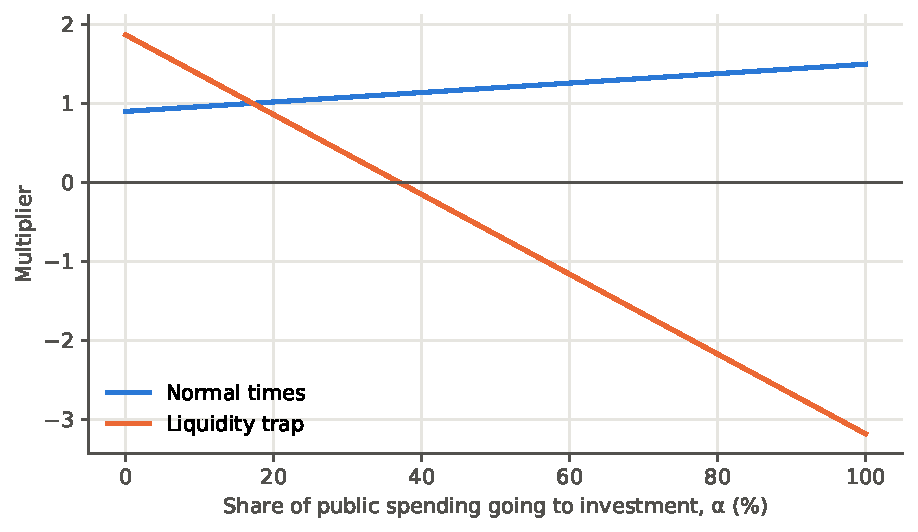
\includegraphics[width=0.8\textwidth]{figure_4_1}
\numfigure{4.1}{Multiplier as a function of $\alpha$, financing of the stimulus plan by lump-sum tax}
\end{figure}

\begin{figure}[htbp]
\centering
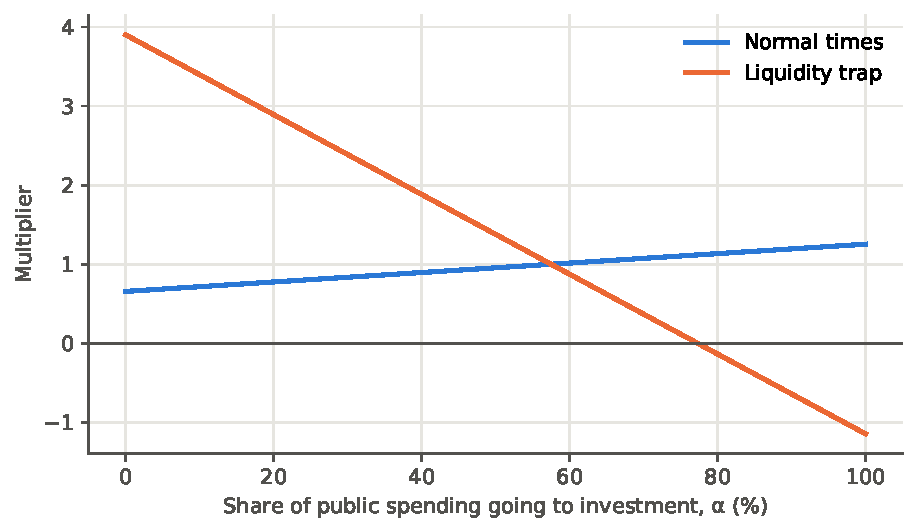
\includegraphics[width=0.8\textwidth]{figure_4_2}
\numfigure{4.2}{Multiplier as a function of $\alpha$, financing of the stimulus plan by labor income tax}
\end{figure}

\section{General case}

The simplifying assumptions according to which public capital becomes productive immediately and depreciation is complete prove unrealistic, even though the previous results are useful for understanding the intuition behind the impact of the liquidity trap and the type of financing on the multiplier. In this section, we relax the assumptions of the previous section. In particular, we consider a non-zero depreciation rate $\delta$ and different times to build public capital, notably $\T = 1$ and $\T = 16$.

In this more general context, we generate a liquidity trap by introducing a shock to liquidity preference in the household utility function. This shock has the effect of increasing household saving in risk-free assets. To simplify the analysis, we assume that the function $F(.)$ is linear. We choose the size of the shock and its persistence so that the liquidity trap lasts 12 quarters. The model is solved using Dynare, assuming that there is no uncertainty (perfect foresight).

Since the dynamic dimension becomes important again in the general version of the model, we present present-value multipliers (\emph{PVM}), which make it possible to measure the total change in output over time. PVMs are frequently used in the literature and can be presented as follows:
\begin{align}
PVM &= \frac{\Et\sum_{t=0}^{h}(1+r_\beta)^{-t}(y_t - y)}{\Et\sum_{t=0}^{h}(1+r_\beta)^{-t}(g_t - g)} \quad \text{(normal times)} \tag{55}\\
\intertext{and}
PVM &= \frac{\Et\sum_{t=0}^{h}(1+r_\beta)^{-t}\Delta y_t}{\Et\sum_{t=0}^{h}(1+r_\beta)^{-t}\Delta g_t} \quad \text{(liquidity trap)} \tag{56}
\end{align}
where $\Delta y_t$ and $\Delta g_t$ measure the difference between the scenario with a simultaneous shock to government spending and liquidity preference and the scenario with only a liquidity preference shock. We first address the case where government spending is financed solely by a labor income tax. In the next section, we introduce public debt.

We maintain the calibration described in Table 4.1. The additional parameters are calibrated as follows: $\delta = 0.025$, $\phi_y = 0.05$, $\rho_\zeta = 0.95$, and $\rho_n = 0.5$ (see Sims and Wolff, 2018).

\subsection{Model without debt}

In this subsection, we present the impact multipliers and the multipliers discounted over 500 periods for the two types of financing of the stimulus plan. Tables 5.1 and 5.2 thus present the multipliers in normal times and in a liquidity trap for different times to build public capital. In addition, we present these multipliers when all government spending is devoted to investment ($\alpha = 1$) and when it is devoted exclusively to consumption ($\alpha = 0$).

\newcommand{\multtable}[9]{%
\begin{tabular}{llccc}
\toprule
& & $\alpha = 0$ & \multicolumn{2}{c}{$\alpha = 1$}\\
& & & $\T = 1$ & $\T = 16$\\
\midrule
\multirow{2}{*}{\textbf{Impact}} & Normal times & #1 & #2 & #3\\
 & Liquidity trap & #4 & #5 & #6\\
\multirow{2}{*}{\textbf{\emph{PVM} over 500 periods}} & Normal times & #7 & #8 & #9\\
}

\begin{table}[htbp]
\centering
\numtable{5.1}{Present-value multipliers, financing of the stimulus plan by lump-sum tax}
\multtable{0.8}{0.92}{0.76}{0.93}{0.95}{1.05}{0.8}{1.89}{1.80}
 & Liquidity trap & 0.93 & 1.88 & 2.20\\
\bottomrule
\end{tabular}
\end{table}

\begin{table}[htbp]
\centering
\numtable{5.2}{Present-value multipliers, financing of the stimulus plan by labor income tax}
\multtable{0.55}{0.67}{0.51}{0.76}{0.75}{0.92}{0.54}{1.63}{1.55}
 & Liquidity trap & 0.84 & 1.76 & 2.11\\
\bottomrule
\end{tabular}
\end{table}

Let us first consider the case $\alpha = 0$. In normal times, when the stimulus plan is financed by a lump-sum tax (Table 5.1), we obtain a multiplier of 0.8 on impact and when discounted over 500 periods. For labor income tax financing (Table 5.2), the multiplier is 0.55 on impact and 0.54 when discounted over 500 periods.

An increase in government spending allocated to consumption causes an increase in aggregate demand and hence in inflation. The monetary authorities therefore raise the nominal interest rate. Since the share of government spending devoted to investment is zero, the spending shock has no deflationary effect that would counter the rise in the interest rate and thus produce a higher fiscal multiplier.

In a liquidity trap, when the stimulus plan is financed by a lump-sum tax (Table 5.1), the multiplier is 0.93 on impact and when discounted over 500 periods. For labor income tax financing (Table 5.2), the multiplier is 0.76 on impact and 0.84 when discounted over 500 periods. The great difference from the normal-times context is that the interest rate set by the monetary authorities is held at zero for several periods. The increase in inflation is thus no longer offset by an increase in the nominal interest rate. As a result, the real interest rate falls and output is stimulated more than in normal times, which explains why multipliers are higher.

Since the government spending of the stimulus plan is not devoted to public capital, households do not anticipate any gain in productivity and hence in wealth, which limits the increase in consumption and thus the multiplier. This is why multipliers are higher when $\alpha$ is non-zero and there is a delay in building capital.

\begin{figure}[htbp]
\centering
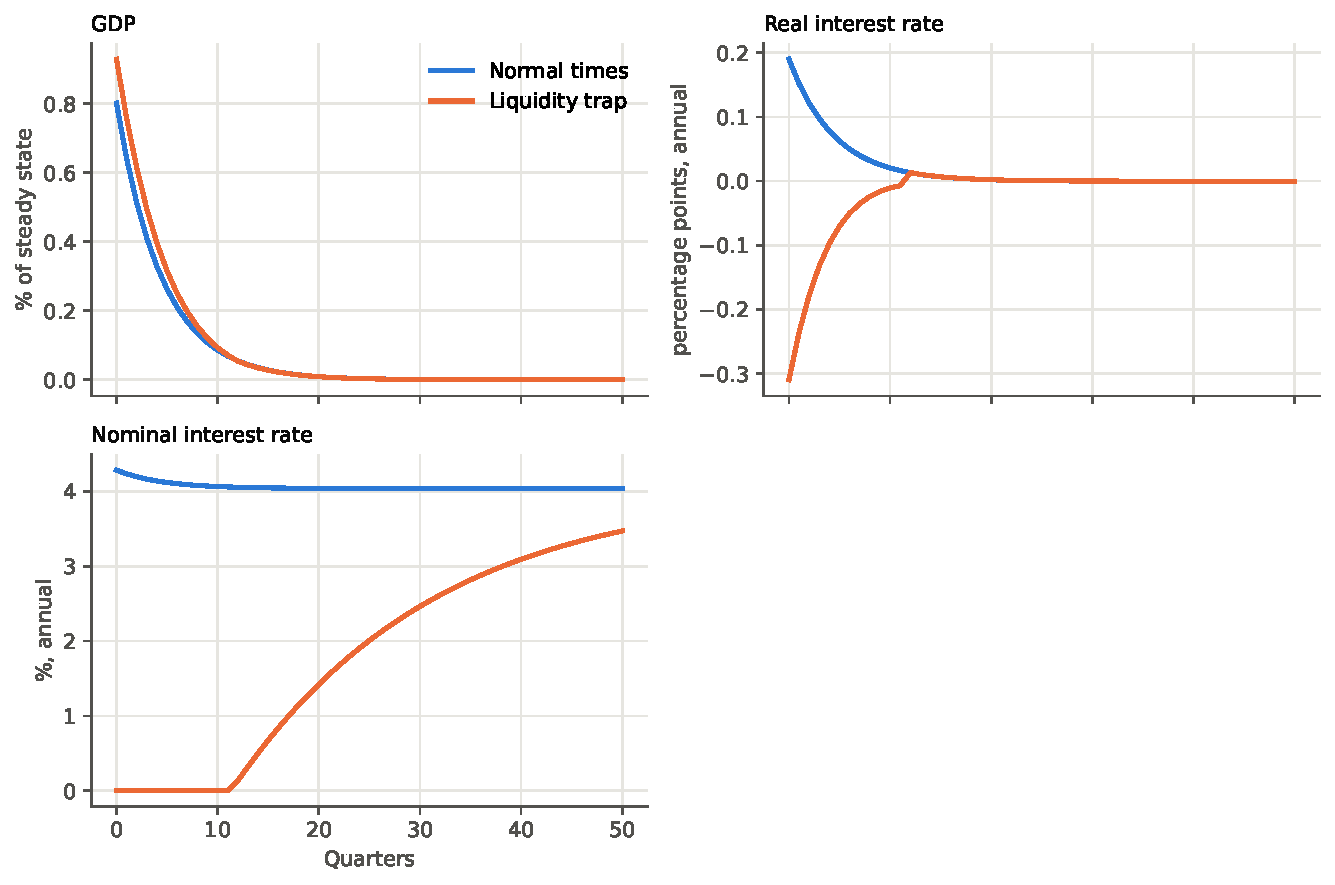
\includegraphics[width=\textwidth]{figure_5_1}
\numfigure{5.1}{Responses to a government spending shock when $\alpha = 0$, lump-sum tax financing}
\end{figure}

\begin{figure}[htbp]
\centering
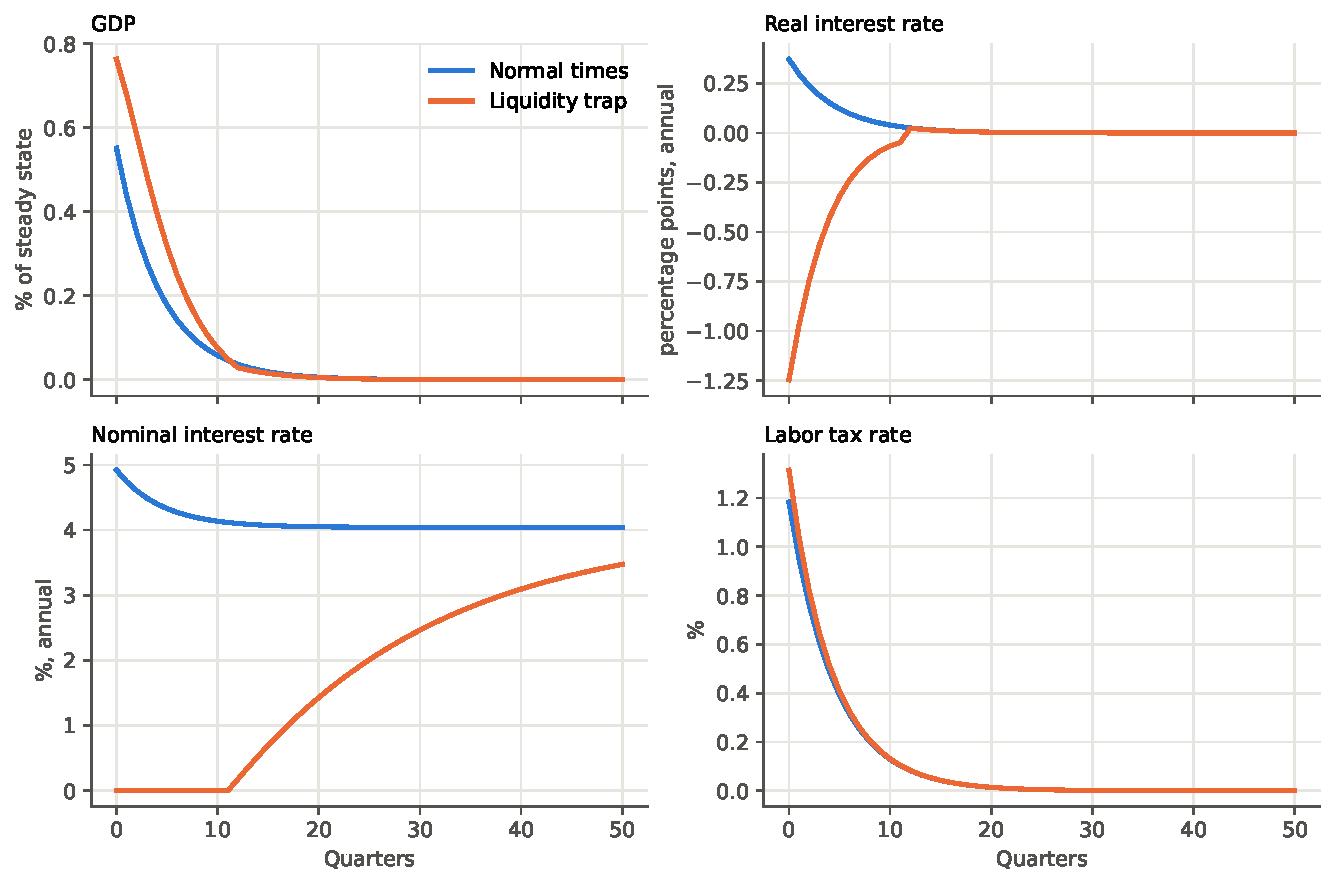
\includegraphics[width=\textwidth]{figure_5_2}
\numfigure{5.2}{Responses to a government spending shock when $\alpha = 0$, labor income tax financing}
\end{figure}

In normal times, and when the stimulus plan is financed by a labor income tax (Figure 5.2), the real interest rate rises more than under lump-sum tax financing (Figure 5.1). Multipliers are therefore lower in the case of labor income tax financing.

In a liquidity trap, we note that in the case of labor income tax financing, the real interest rate falls much more than under lump-sum tax financing, given the inflationary effect of the labor income tax, which, as we recall, is a distortionary tax. This explains why the difference between the multiplier in a trap and in normal times is larger for labor income tax financing. The multipliers corresponding to lump-sum tax financing are nevertheless larger in a trap than in the case of labor income tax financing.

Let us now analyze the case where $\alpha = 1$ and the time to build capital is 1 quarter. In normal times, when the stimulus plan is financed by a lump-sum tax (Table 5.1), we obtain a multiplier of 0.92 on impact and of 1.89 for the value discounted over 500 periods. For labor income tax financing (Table 5.2), the multiplier is 0.67 on impact and 1.63 when discounted over 500 periods. The multipliers are higher than in the previous case.

Since all the government spending of the stimulus plan is devoted to investment in capital, the spending shock will have the effect of lowering marginal costs, which exerts a deflationary pressure. This effect arrives relatively quickly since the time to build is only one quarter. The increase in the nominal interest rate described in the previous case is thus largely reduced, which has a positive effect on output.

In a liquidity trap, when the stimulus plan is financed by a lump-sum tax (Table 5.1), the multiplier is 0.95 on impact and 1.88 when discounted over 500 periods. For labor income tax financing (Table 5.2), the multiplier is 0.75 on impact and 1.76 when discounted over 500 periods.

The intuition behind the fact that the multiplier in a trap is higher than in normal times remains similar to what has already been described. In a liquidity trap, any inflationary pressure pushes the multiplier upward. Given the construction of public capital, households anticipate gains in productivity and hence in wealth. This is all the more so the longer the time to build, which is why, when the time to build is too short, it is not impossible to observe a lower multiplier in a trap than in normal times.

\begin{figure}[htbp]
\centering
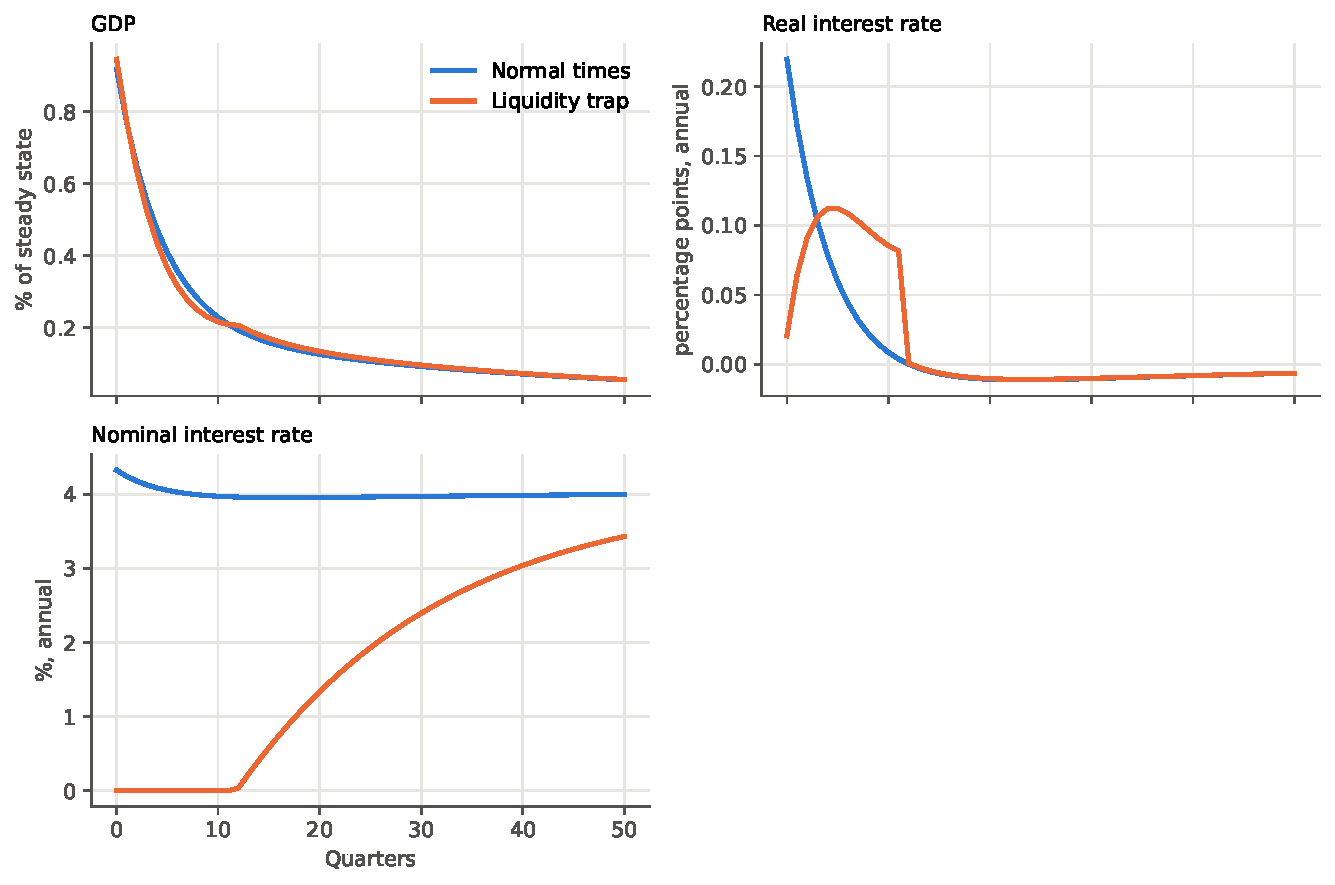
\includegraphics[width=\textwidth]{figure_5_3}
\numfigure{5.3}{Responses to a public investment shock when $\alpha = 1$ and $\T = 1$, lump-sum tax financing}
\end{figure}

\begin{figure}[htbp]
\centering
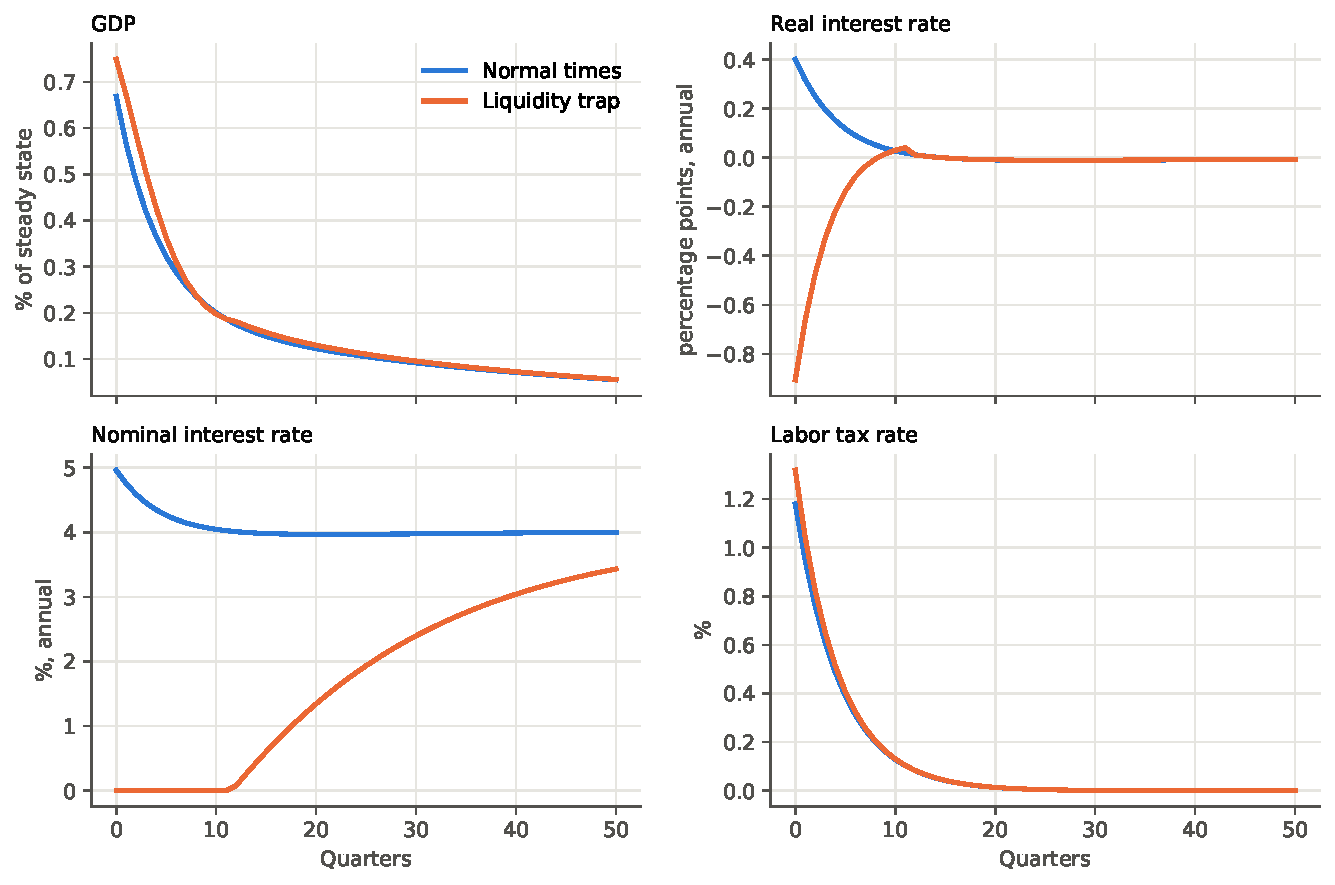
\includegraphics[width=\textwidth]{figure_5_4}
\numfigure{5.4}{Responses to a public investment shock when $\alpha = 1$ and $\T = 1$, labor income tax financing}
\end{figure}

For lump-sum tax financing (Figure 5.3), inflationary pressures are not strong enough to make the real interest rate fall initially when the time to build capital is 1 quarter. By contrast, in the case of labor income tax financing (Figure 5.4), there is much more inflationary pressure given the labor income tax, so the multiplier in a trap is higher than in normal times. However, multipliers for lump-sum financing are higher than with labor income tax financing because of the persistent fall in the real interest rate on exit from the trap in the first case.

Let us now analyze the case where $\alpha = 1$ and the time to build capital is 16 quarters. In normal times, when the stimulus plan is financed by a lump-sum tax (Table 5.1), we obtain a multiplier of 0.76 on impact and of 1.80 for the value discounted over 500 periods. For labor income tax financing (Table 5.2), the multiplier is 0.51 on impact and 1.55 when discounted over 500 periods. In a liquidity trap, when the stimulus plan is financed by a lump-sum tax (Table 5.1), the multiplier is 1.05 on impact and 2.20 when discounted over 500 periods. For labor income tax financing (Table 5.2), the multiplier is 0.92 on impact and 2.11 when discounted over 500 periods.

It is interesting to observe that when the time to build is longer, in this case 16 quarters, the fiscal multiplier tends to fall in normal times while it rises in a liquidity trap. Indeed, when the time to build is long, the productivity gains anticipated by agents occur very far in the future, and therefore do not have as much effect on current aggregate demand, thereby reducing the fiscal multiplier in normal times. In a liquidity trap, this effect is more than offset by the delay in the disinflationary effect resulting from the fall in future marginal cost, which amplifies the multiplier.

\begin{figure}[htbp]
\centering
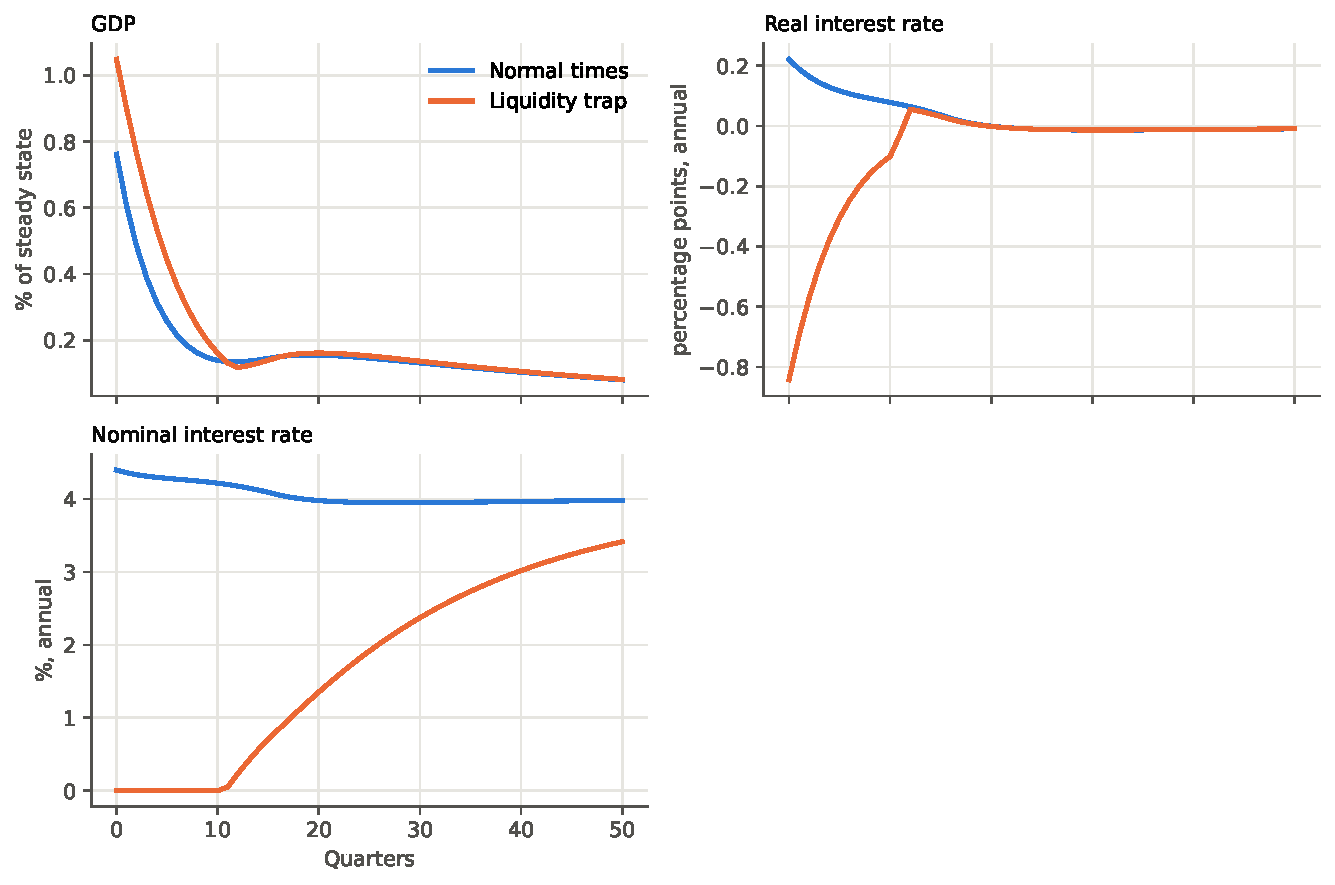
\includegraphics[width=\textwidth]{figure_5_5}
\numfigure{5.5}{Responses to a public investment shock when $\alpha = 1$ and $\T = 16$, lump-sum financing}
\end{figure}

\begin{figure}[htbp]
\centering
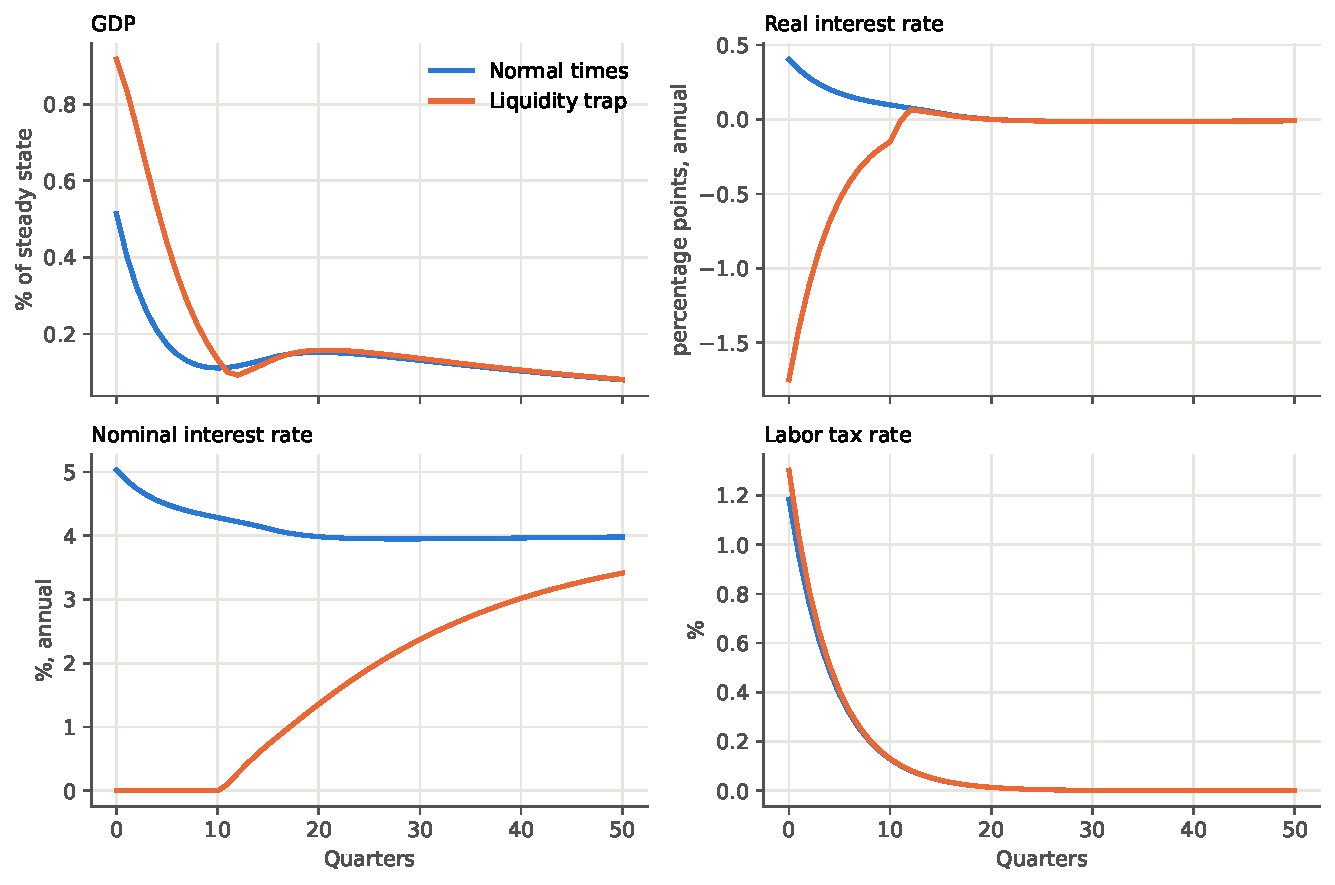
\includegraphics[width=\textwidth]{figure_5_6}
\numfigure{5.6}{Responses to a public investment shock when $\alpha = 1$ and $\T = 16$, labor income tax financing}
\end{figure}

One point that remains to be discussed in this section is the fact that the multipliers under lump-sum tax financing are higher than under labor income tax financing in a liquidity trap, regardless of the share of spending devoted to capital and the time to build. This seems to contradict what we found in the algebraic solution. This can be explained by the process of the labor income tax, which differs from the case of the solution of the linear model. In the algebraic solution, we considered a Markov process on $\beta_t$ to generate the liquidity trap. As a consequence, on exit from the trap, all the variables of the model returned immediately to their steady state, including the labor income tax, since this version of the model had no endogenous state variable. This is not the case in the general version of the model, where the exit from the trap is endogenous. Indeed, after a liquidity preference shock, the labor income tax remains higher than its initial (zero) level even once the economy has exited the trap, and only returns to that level very gradually (see Figures 5.2, 5.4, and 5.6). Agents therefore anticipate a fall in their future after-tax income relative to a situation where the tax would be zero, which negatively affects the fiscal multiplier.

The path of the labor income tax is therefore decisive for the size of the multiplier. In the next section, with the addition of debt, we will be able to shed more light on this question.

\subsection{Model with debt}

We now arrive at the most elaborate version of our model, in which government spending is financed by a lump-sum tax, a labor income tax, and debt. Recall that the labor income tax adjusts to past debt according to a process inspired by Sims and Wolff (2018):
\begin{equation*}
\tau_t = (1-\rho_n)\tau + \rho_n\tau_{t-1} + (1-\rho_n)\gamma_n\left(\frac{B_t}{Y_t} - \frac{B}{Y}\right)
\end{equation*}
which was already described in Section 3. We choose $\gamma_n$ such that the debt-to-GDP ratio is not explosive. We set $\gamma_n = 0.1$ and $\rho_n = 0.5$ as in Sims and Wolff (2018). It is through the parameter $\gamma_n$ that we can adjust the path of the tax in a liquidity trap, so it will be interesting to carry out a sensitivity analysis on this parameter. As before, we will calculate the fiscal multiplier in normal times, in a liquidity trap, and for different times to build public capital. We consider only the case where the tax and the debt are zero at the steady state, in order to be able to compare with the multipliers obtained previously.

\begin{table}[htbp]
\centering
\numtable{6.1}{Multipliers with debt financing and $\gamma_n = 0.1$}
\multtable{0.63}{0.75}{0.58}{0.98}{0.99}{1.10}{0.07}{1.16}{1.07}
 & Liquidity trap & 0.57 & 1.54 & 1.81\\
\bottomrule
\end{tabular}
\end{table}

Impact multipliers in normal times fall relative to the case of financing exclusively by labor income tax. By contrast, in a liquidity trap, the multipliers are larger. This suggests that it may be possible to reconcile our results with those obtained algebraically by varying $\gamma_n$, which plays a decisive role in the path of the tax. We therefore carry out a sensitivity analysis on the parameter $\gamma_n$ when $\alpha = 1$ and the time to build public capital is 16 quarters. Since the values considered must remain consistent with estimates in the literature, we vary $\gamma_n$ over the interval $[0.05; 0.25]$.

\begin{figure}[htbp]
\centering
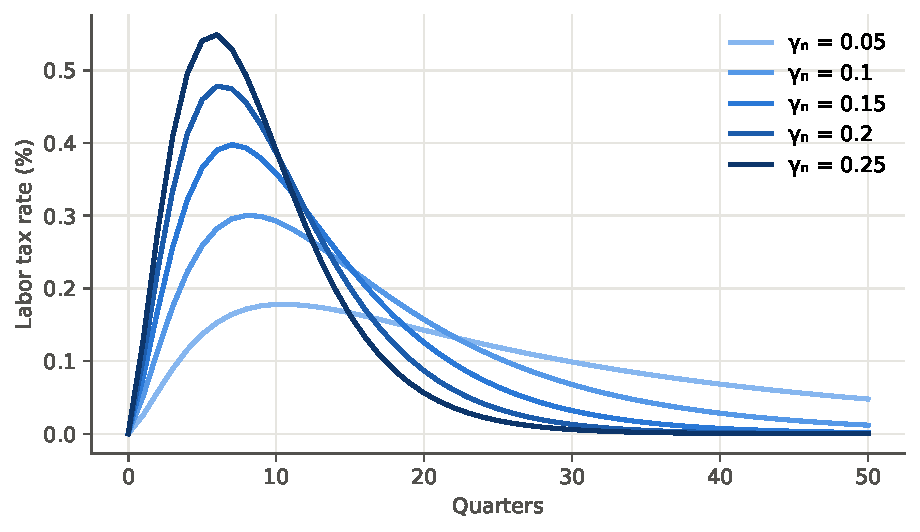
\includegraphics[width=0.8\textwidth]{figure_6_1}
\numfigure{6.1}{Path of the labor income tax as a function of $\gamma_n$ in a liquidity trap during a government spending shock}
\end{figure}

\begin{table}[htbp]
\centering
\numtable{6.2}{Multipliers in a liquidity trap when $\T = 16$}
\begin{tabular}{ccc}
\toprule
$\gamma_n$ & Impact multiplier & PVM over 500 periods\\
\midrule
0.05 & 1.05 & 1.65\\
0.1 & 1.10 & 1.81\\
0.15 & 1.15 & 1.96\\
0.2 & 1.18 & 2.08\\
0.25 & 1.20 & 2.15\\
\bottomrule
\end{tabular}
\end{table}

We thus note that the higher $\gamma_n$ is, the less persistent the tax is and the higher the levels it reaches in a trap (see Figure 6.1), thereby increasing the value of the multiplier. There would thus exist a level of $\gamma_n$ that strikes a compromise between the level and persistence of the tax in a liquidity trap, such that the fiscal multiplier is higher than with lump-sum tax financing. On impact, this is the case as soon as $\gamma_n$ exceeds the threshold of 0.05. For the PVM, the minimum required value of $\gamma_n$ is slightly above the maximum bound considered (0.25).

\section{Conclusion}

In this thesis, we compared the fiscal multiplier across different types of financing of a stimulus plan within a single model with a unique steady state. Varying the type of government spending financing only away from the steady state allowed us to make an analytical comparison of multipliers in normal times and in a liquidity trap by considering a static linear model, and then to determine whether, and in what context, the analytical results hold in a dynamic non-linear model.

Our results highlight the importance of the financing method for the size of the multiplier. Our main conclusion is that, insofar as the increase in the labor income tax takes place mainly while the economy is in a liquidity trap but is reversed as soon as the economy has exited the trap, it is possible to have a fiscal multiplier comparable (and potentially superior) to that corresponding to lump-sum tax financing.

It would now be interesting in future research to extend the model presented in this thesis to take account of other types of distortionary taxes such as the consumption tax or the tax on capital income. Also, to complete the literature, it would be relevant to determine optimal fiscal policy in an economy that has several fiscal instruments but in which the government is constrained to follow pre-established fiscal rules.

\newpage
\section*{Bibliography}
\addcontentsline{toc}{section}{Bibliography}
\begin{list}{}{\setlength{\leftmargin}{2em}\setlength{\itemindent}{-2em}\setlength{\itemsep}{0.3em}}
\small
\item Aloui, R. and A. Eyquem (2019). ``Spending multipliers with distortionary taxes: Does the level of public debt matter?'', \emph{Journal of Macroeconomics}, vol. 60, p. 275-293.
\item Altig, D., L. J. Christiano, M. Eichenbaum and J. Linde (2011). ``Firm-specific capital, nominal rigidities and the business cycle'', \emph{Review of Economic Dynamics}, vol. 14, no. 2, p. 225-247.
\item Auerbach, Alan, J and Yuriy Gorodnichenko (2012). ``Measuring the output responses to fiscal policy'', \emph{American Economic Journal: Economic Policy}, vol. 4, p. 1-27.
\item Barro, R. J. (1981). ``Output effects of government purchases'', \emph{Journal of Political Economy}, vol. 89, no. 6, p. 1086-1121.
\item Barro, Robert J (1974). ``Are government bonds net wealth?'', \emph{J.P.E}, vol. 82, p. 1095-1117.
\item Bom, P. R. D. and J. E. Ligthart (2014). ``What have we learned from three decades of research on the productivity of public capital?'', \emph{Journal of Economic Surveys}, vol. 28, no. 5, p. 889-916.
\item Boehm, C. (2020). ``Government consumption and investment: Does the composition of purchases affect the multiplier?'', \emph{Journal of Monetary Economics}, vol. 115, p. 80-93.
\item Bouakez, H., M. Guillard and J. Roulleau-Pasdeloup (2017). ``Public investment, time to build, and the zero lower bound'', \emph{Review of Economic Dynamics}, vol. 23, p. 60-79.
\item Bouakez, H., M. Guillard and J. Roulleau-Pasdeloup (2020). ``The optimal composition of public spending in a deep recession'', \emph{Journal of Monetary Economics}, vol. 114, p. 330-349.
\item Bouakez, H. and M. Normandin (2014). ``Measuring the effects of fiscal policy'', \emph{Journal of Economic Dynamics and Control}, vol. 47, p. 123-151.
\item Calvo, G. A. (1983). ``Staggered prices in a utility-maximizing framework'', \emph{Journal of Monetary Economics}, vol. 12, no. 3, p. 383-398.
\item Christiano, L., M. Eichenbaum and S. Rebelo (2011). ``When is the government spending multiplier large?'', \emph{Journal of Political Economy}, vol. 119, no. 1, p. 78-121.
\item Eggertsson, G. B. (2011). ``What fiscal policy is effective at zero interest rates?'', \emph{NBER Macroeconomics Annual}, vol. 25.
\item Eggertsson, Gauti B. and Michael Woodford (2004). ``Policy options in a liquidity trap'', \emph{American Economic Review}, vol. 94, p. 76-79.
\item Fischer, S. (1977). ``Long-term contracts, rational expectations, and optimal money supply rule'', \emph{Journal of Political Economy}, vol. 85, no. 1, p. 191-205.
\item Gal\'i, Jordi and MyiLibrary (2008). \emph{Monetary policy, inflation, and the business cycle: An introduction to the new keynesian framework}, Princeton, N.J, Princeton University Press.
\item Jord\`a, \`O. (2005). ``Estimation and Inference of Impulse Responses by Local Projections'', \emph{American Economic Review}, vol. 95, no. 1, p. 161-182.
\item Keynes (1936). \emph{The general theory of employment interest and money}.
\item Kydland, F. E. and E. C. Prescott (1982). ``Time to build and aggregate fluctuations'', \emph{Econometrica}, vol. 50, no. 6, p. 1345-1370.
\item Lemoine, M. and J. Lind\'e (2023). ``Fiscal stimulus in liquidity traps: Conventional or unconventional policies?'', \emph{European Economic Review}, vol. 151.
\item Lucas, R. E. (1976). ``Econometric policy evaluation - critique'', \emph{Carnegie-Rochester Conference Series on Public Policy}, vol. 1, p. 19-46.
\item McCulloch (1846). \emph{The works of david ricardo}, London, John Murray.
\item Miyamoto, W., TL. Nguyen and D. Sergeyev (2018). ``Government spending multipliers under the zero lower bound: Evidence from japan.'', \emph{American Economic Journal-Macroeconomics}, vol. 10, no. 3.
\item Nakata, Taisuke (2017). ``Optimal government spending at the zero lower bound: A non-ricardian analysis'', \emph{Review of Economic Dynamics}, vol. 23, p. 150-169.
\item Perotti, R (2004). ``Public Investment: Another (Different) Look'', IGIER, Working Paper no. 277, p. 49.
\item Ramey, V. A. (2011). ``Identifying government spending shocks: It's all in the timing'', \emph{Quarterly Journal of Economics}, vol. 126, no. 1, p. 1-50.
\item Ramey, V. A. (2019). ``Ten years after the financial crisis: What have we learned from the renaissance in fiscal research?'', \emph{Journal of Economic Perspectives}, vol. 33, no. 2, p. 89-114.
\item Ramey, V. A. (2020). ``The macroeconomic consequences of infrastructure investment'', National Bureau of Economic Research.
\item Ramey, V. A. and M. D. Shapiro (1998). ``Costly capital reallocation and the effects of government spending'', \emph{Carnegie-Rochester Conference Series on Public Policy}, vol. 48, p. 145-194.
\item Ramey, V. A. and S. Zubairy (2018). ``Government spending multipliers in good times and in bad: Evidence from us historical data'', \emph{Journal of Political Economy}, vol. 126, no. 2, p. 850-901.
\item Sims, E and J. Wolff (2018). ``The output and welfare effects of government spending shocks over the business cycle'', \emph{International Economic Review}, vol. 59, no. 3, p. 1403-1435.
\item Woodford, M. (2011). ``Simple analytics of the government expenditure multiplier'', \emph{American Economic Journal-Macroeconomics}, vol. 3, no. 1, p. 1-35.
\end{list}

\newpage
\appendix
\section*{Annex A: Steady state}
\addcontentsline{toc}{section}{Annex A: Steady state}

To solve for the steady state, we will use two particularly useful identities
\begin{equation}
\frac{Y}{C} = \frac{1}{1-\gbar} \tag{1}
\end{equation}
and
\begin{equation}
G = \frac{\gbar}{1-\gbar}C \tag{2}
\end{equation}

\subsection*{Marginal cost}

The steady state of marginal cost can be calculated from the first-order condition of the intermediate-goods producers
\begin{equation*}
MC = \frac{\theta}{\theta-1} + \frac{\Psi}{\theta}\pi(1+\pi) - \frac{\Psi}{\theta}\frac{U_c}{U_c}\frac{Y}{Y}\pi(1+\pi)
\end{equation*}
Since inflation is zero at the steady state, we easily obtain steady-state marginal cost:
\begin{equation*}
\boldsymbol{MC = \frac{\theta}{\theta-1}}
\end{equation*}

\subsection*{Labor}

Labor at the steady state can be calculated using the supply and demand equations:
\begin{align*}
w &= \frac{-U_N}{U_C(1-\tau)}\\
w &= MC.F_N
\end{align*}
where $\frac{-U_N}{U_C} = \frac{1-\gamma}{1-N}\frac{C}{\gamma}$ and $F_N = a\frac{F}{N}$. We therefore have
\begin{equation*}
\frac{1}{(1-\tau)}\frac{1-\gamma}{1-N}\frac{C}{\gamma} = aMC\frac{F}{N}
\end{equation*}
By replacing $MC$ with $\frac{\theta}{\theta-1}$ and using the fact that $\frac{F}{C} = \frac{Y}{C} = \frac{a}{1-g}$, we can isolate $N$ and express it as a function of the model's parameters:
\begin{equation*}
\boldsymbol{N = \left(\frac{1-\gamma}{\gamma}\frac{1}{1-\tau}\frac{1-g}{a}\frac{\theta-1}{\theta} + 1\right)^{-1}}
\end{equation*}

\subsection*{Consumption}

Thanks to the capital accumulation law, equation (19), we can define
\begin{equation*}
\delta K = G^i = \abar G
\end{equation*}
We therefore have
\begin{equation*}
K = \frac{\abar}{\delta}G
\end{equation*}
Using identity (2) we have:
\begin{equation*}
K = \frac{\abar g}{1-g}C
\end{equation*}
In addition, we have:
\begin{equation*}
Y = N^a K^b
\end{equation*}
Using identity (1), we can express $C$ as a function of $N$ and $K$:
\begin{equation*}
C = (1-\gbar)N^a K^b
\end{equation*}
Now, by expressing $K$ as a function of $C$, we can express $C$ as a function of $N$ and the model's parameters:
\begin{equation*}
\boldsymbol{C = \left((1-g)N^a\left(\frac{\abar g}{1-g}\right)^b\right)^{\frac{b}{1-b}}}
\end{equation*}
From there, it is enough to substitute the values of $N$ and $C$ into the equations that contain them to obtain:
\begin{align*}
\boldsymbol{K} &\boldsymbol{= \frac{\abar g}{1-g}C}\\
\boldsymbol{G} &\boldsymbol{= \frac{\delta K}{\abar}}\\
\boldsymbol{W} &\boldsymbol{= \frac{1-\gamma}{\gamma}\frac{C}{1-N}\frac{1}{1-\tau}}\\
\boldsymbol{Y} &\boldsymbol{= C+G}
\end{align*}

\subsection*{Nominal interest rate}

In line with the literature, we set the nominal interest rate as follows:
\begin{equation*}
\boldsymbol{i = \frac{1}{\beta} - 1}
\end{equation*}

\subsection*{Labor income tax}

To have one and the same steady state in all cases, we set the labor income tax to zero.
\begin{equation*}
\boldsymbol{\tau = 0}
\end{equation*}

\subsection*{Debt}

At the steady state we have:
\begin{equation*}
G + iB \leq T + \tau WN
\end{equation*}
We also know that at the steady state $T = G$, in order to have the same steady state as under lump-sum tax financing of the stimulus plan. We then have:
\begin{equation*}
\boldsymbol{\frac{B}{P} = \frac{\tau WN}{i} = 0}
\end{equation*}
where $i = \frac{1}{\beta} - 1$.

\newpage
\section*{Annex B: Dynare code}
\addcontentsline{toc}{section}{Annex B: Dynare code}

\subsection*{Case without debt}
\lstinputlisting{annex_b_nodebt.mod}

\subsection*{Case with debt}
\lstinputlisting{annex_b_debt.mod}

\end{document}
